\documentclass[crop,tikz]{standalone}%

\usetikzlibrary{matrix,calc,positioning}

\begin{document}

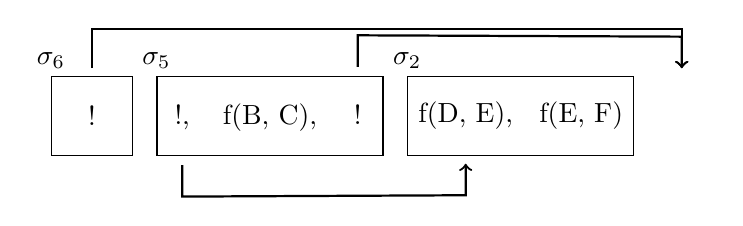
\begin{tikzpicture}[baseline]

\matrix (outer) [matrix of nodes,
                 nodes={draw, minimum width=0.5cm, minimum height=1cm, anchor=center},
                 column sep=0.3cm, row sep=0.3cm] {
\phantom{AAA} & \phantom{AAAAAAAAAA} & \phantom{AAAAAAAAAA} &  \node[draw=none] (A) {\phantom{xx}};\\
};

\matrix (inner1) [matrix of nodes,
                 nodes={minimum size=0.6cm},
                 column sep=0.1cm, row sep=0.1cm] at (outer-1-1.center) {
! \\
};

\matrix (inner2) [matrix of nodes,
                 nodes={minimum size=0.6cm},
                 column sep=0.1cm, row sep=0.1cm] at (outer-1-2.center) {
!, & f(B, C), & ! \\
};

\matrix (inner3) [matrix of nodes,
                 nodes={minimum size=0.6cm},
                 column sep=0.1cm, row sep=0.1cm] at (outer-1-3.center) {
f(D, E), & f(E, F) \\
};


\matrix (innerL) [matrix of nodes,
                 nodes={minimum size=0.6cm},
                 column sep=0.1cm, row sep=0.1cm] at (A.center) {
\phantom{x} \\
};

\draw[->, thick]
  ($(inner1-1-1.north)+(0,0.3)$) -- ++(0,0.5)  
  -- ($(innerL-1-1.north)+(0,0.8)$)            
  -- ($(innerL-1-1.north)+(0,0.3)$);           

\draw[->, thick]
  ($(inner2-1-3.north)+(0,0.3)$) -- ++(0,0.4)  
  -- ($(innerL-1-1.north)+(0,0.7)$)            
  -- ($(innerL-1-1.north)+(0,0.3)$);           

\draw[->, thick]
  ($(inner2-1-1.south)-(0,0.3)$) -- ++(0,-0.4)  
  -- ($(inner3-1-1.south)-(0,0.7)$)            
  -- ($(inner3-1-1.south)-(0,0.3)$);           

\node at ($(outer-1-1.north west)+(-0,0.2)$) {$\sigma_6$};
\node at ($(outer-1-2.north west)+(-0,0.2)$) {$\sigma_5$};
\node at ($(outer-1-3.north west)+(-0,0.2)$) {$\sigma_2$};

\end{tikzpicture}

\end{document}
